
\section{In which X-ray energy range can I use the detector?}
What limits the energy range in which the detector can be used is defined both by the sensors characteristics and the readout electronics.

\subsection{Sensors}
Most of the SLS detectors make use of silicon sensors.

Since silicon is a relatively light for hard X-rays the only limitation at high energies is the acceptable absorption efficiency that can be achieved in the sensors thickness.\\
Figure~\ref{fig:effidet} shows the absorption efficiency as a function of the X-ray energy and detector thickness. Normally it is possible to use sensors up to 1~mm thick, while to achieve larger absorption thicknesses it is necessary tu assemble and control telescopic systems (possible up to a few mms).\\
To achieve larger absorption thicknesses, the sensors can be oriented in edge-on configuration (in particular strip sensors). However in this case one should take into consideration the dead entrance window due to the cutting distance from the strips, which is normally several hundreds micron, or even up to mms and reduces the absorption efficiency at lower energies.

\begin{figure}
\caption{Efficiency of a silicon sensor as a function of the sensors thickness and X-ray energy.}\label{fig:effidet}
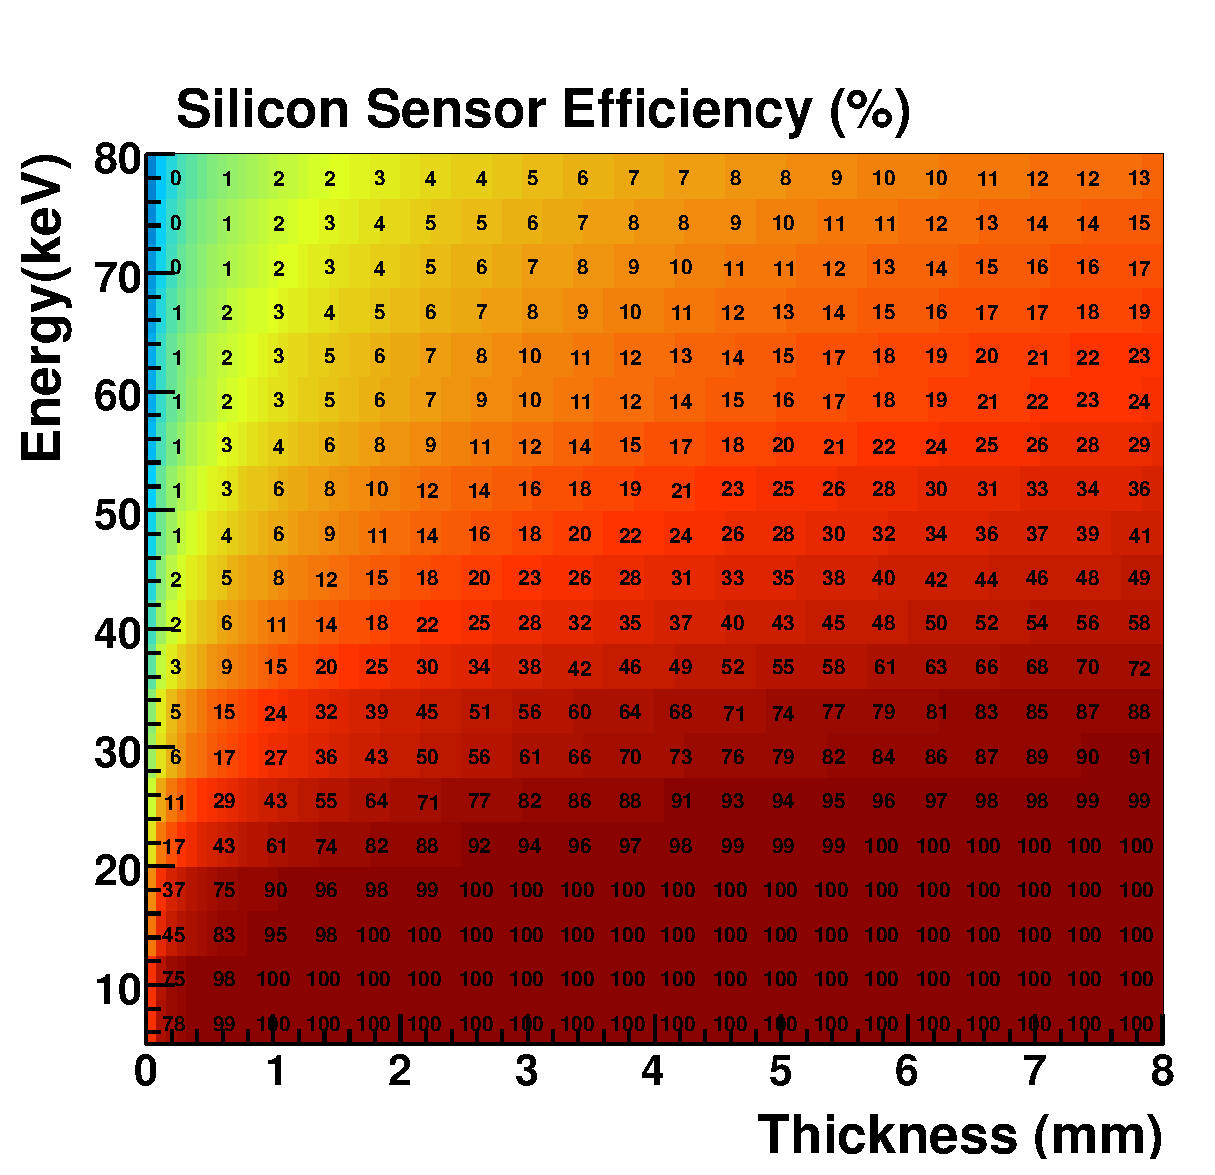
\includegraphics[width=\textwidth]{images/effiSiHardXRays2}
\end{figure} 

In standard face-on orientation, the backplane of the sensor acts as the entrance window. It presents a think n+ doped layer, which is unsensitive to radiation and causes a loss of efficiency at low energies.
Figure~\ref{fig:effiback} shows the absorption efficiency of the sensors for different backplane thicknesses at low energies.\\
The exact thickness of the backplane for standard SLS sensors is not exactly known but should be about 1-2~$\mu$m.

\begin{figure}
\caption{Efficiency of a silicon sensor as a function of the X-ray energy for different thicknesses of the backplane.}\label{fig:effiback}
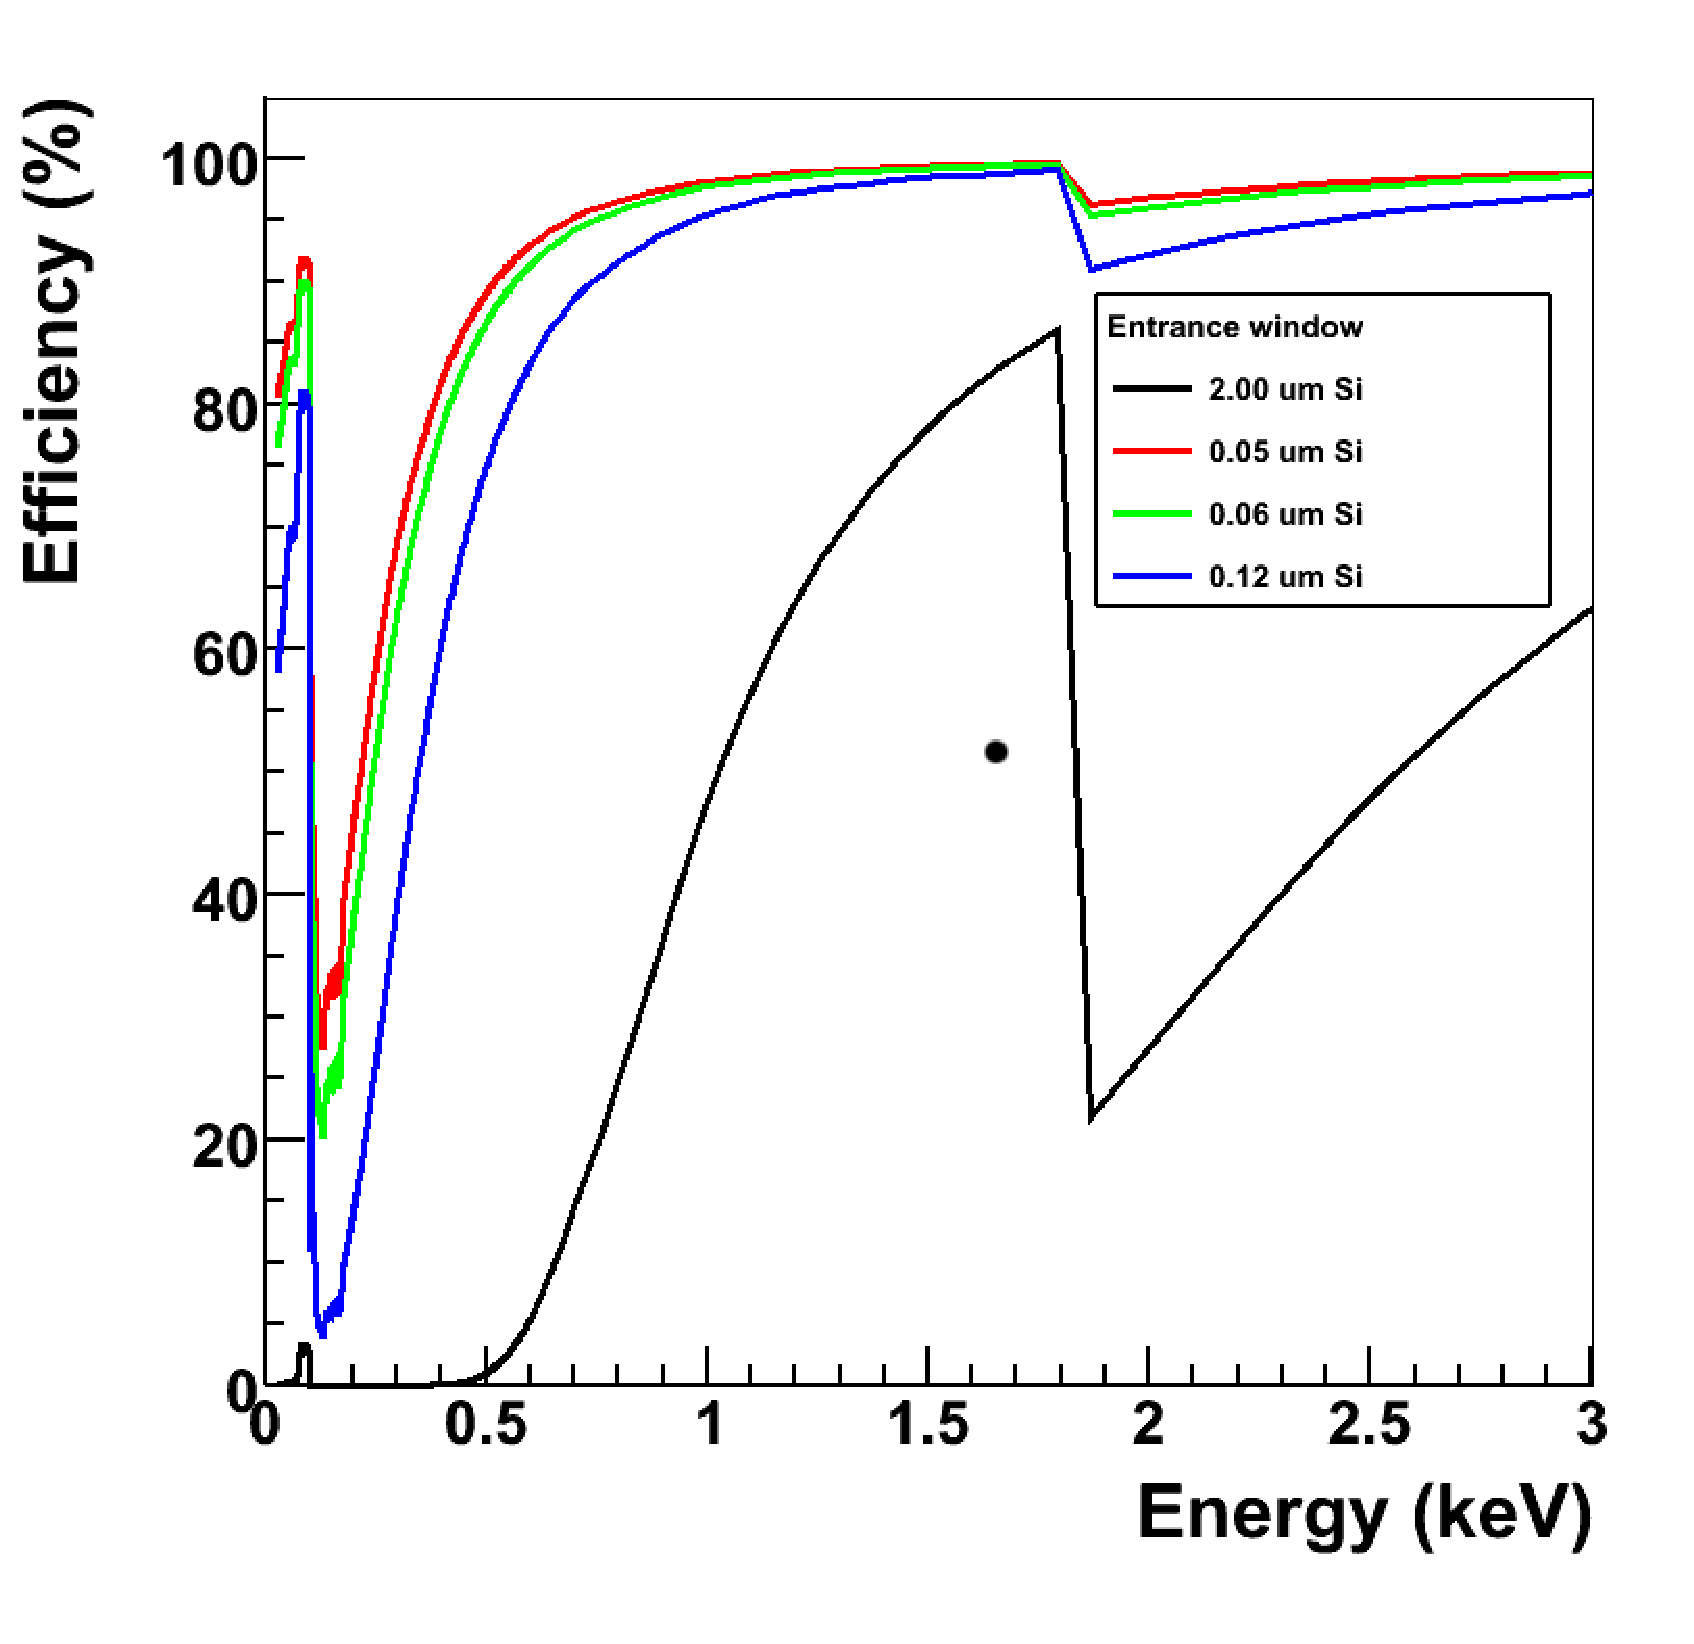
\includegraphics[width=\textwidth]{images/effiThinkBackplanes}
\end{figure} 

However for lower energies, the main limitation is normally given by the noise of the frontend electronics (if single photon resolution is required).\\
For higher energies it is also possible to use different sesnor materials as CdTe or Ge, although up to now they cannot provide the same signal quality as silicon.


\subsection{Frontend electronics}

The limitations on the energy range arising from the readout electronics come from the noise and from saturation. 
The electronic noise  limits the minimum detectable energy for single photons, while saturation limits the maximum detectable signal either for single photons or in total.
\begin{itemize}
\item In \textbf{single photon counting detectors}, the minimum threshold  cannot be set lower than 3-5 times the electronic noise.
If the threshold is set at approximately half of the X-ray energy (see specific documentation about single photon counting detectors), the minimu detectable energy will be about 6-10 times the noise.\\
In order to reduce the noise of the frontend electronics different settings can be chosen, but this puts a limit on the maximum incoming flux that can be detected without incurring in pileup (see specific documentation about single photon counting detectors). Figure~\ref{fig:mythensett} shows an example of the settings used for the MYTHEN detector for different energy ranges and fluxes.\\
For state of the art single photon counting detectors, the minimum thrshold can be about 2-3~keV (details depend on the detector and can be further reduced using special settings).

Concerning saturation, this imposes a maximum value for the comparator threshold. Normally photons of higher energies can still be detected, but without resolution concerning the threshold energy and eventually losing spatial resolution.
By changing the settings it is possible to increase the maximum threshold value (normally also noise increases in this case).

\item For \textbf{charge integrating detectors} the electronics noise puts a limit on the minimum detectable signal. Therefore if single photon resolution is required, the minimum detectable energy is defined as for single photon counting detectors at about 6-10 times the electronic noise. In case no single photon resolution is required, the electronic noise will put a limit on the sensitivity of the detector i.e. the total accumulated signal needs to be larger than 6-10 times the noise in order to be detected (also about 2-3~keV depending on the detector). It is important to point out that the acquisition time of charge integrating detectors is limited by the leakage current of the sesnors and the noise quadratically sums out. Therefore the signal for low energy photons should be strong enough to be acquired during single frames.

Concerning saturation, this sets a limit on the total number of photons acquired during the acquistion slot and is normally much larger than the energy released by single X-rays. Dynamic gain switching can strongly increase the dynamic range of the detector up to 10E+4 12~keV photons. 


\end{itemize}


\begin{figure}
\caption{Settings to be chosen for the MYTHEN detector as a function of the X-ray energy and radiation intensity.}\label{fig:mythensett}
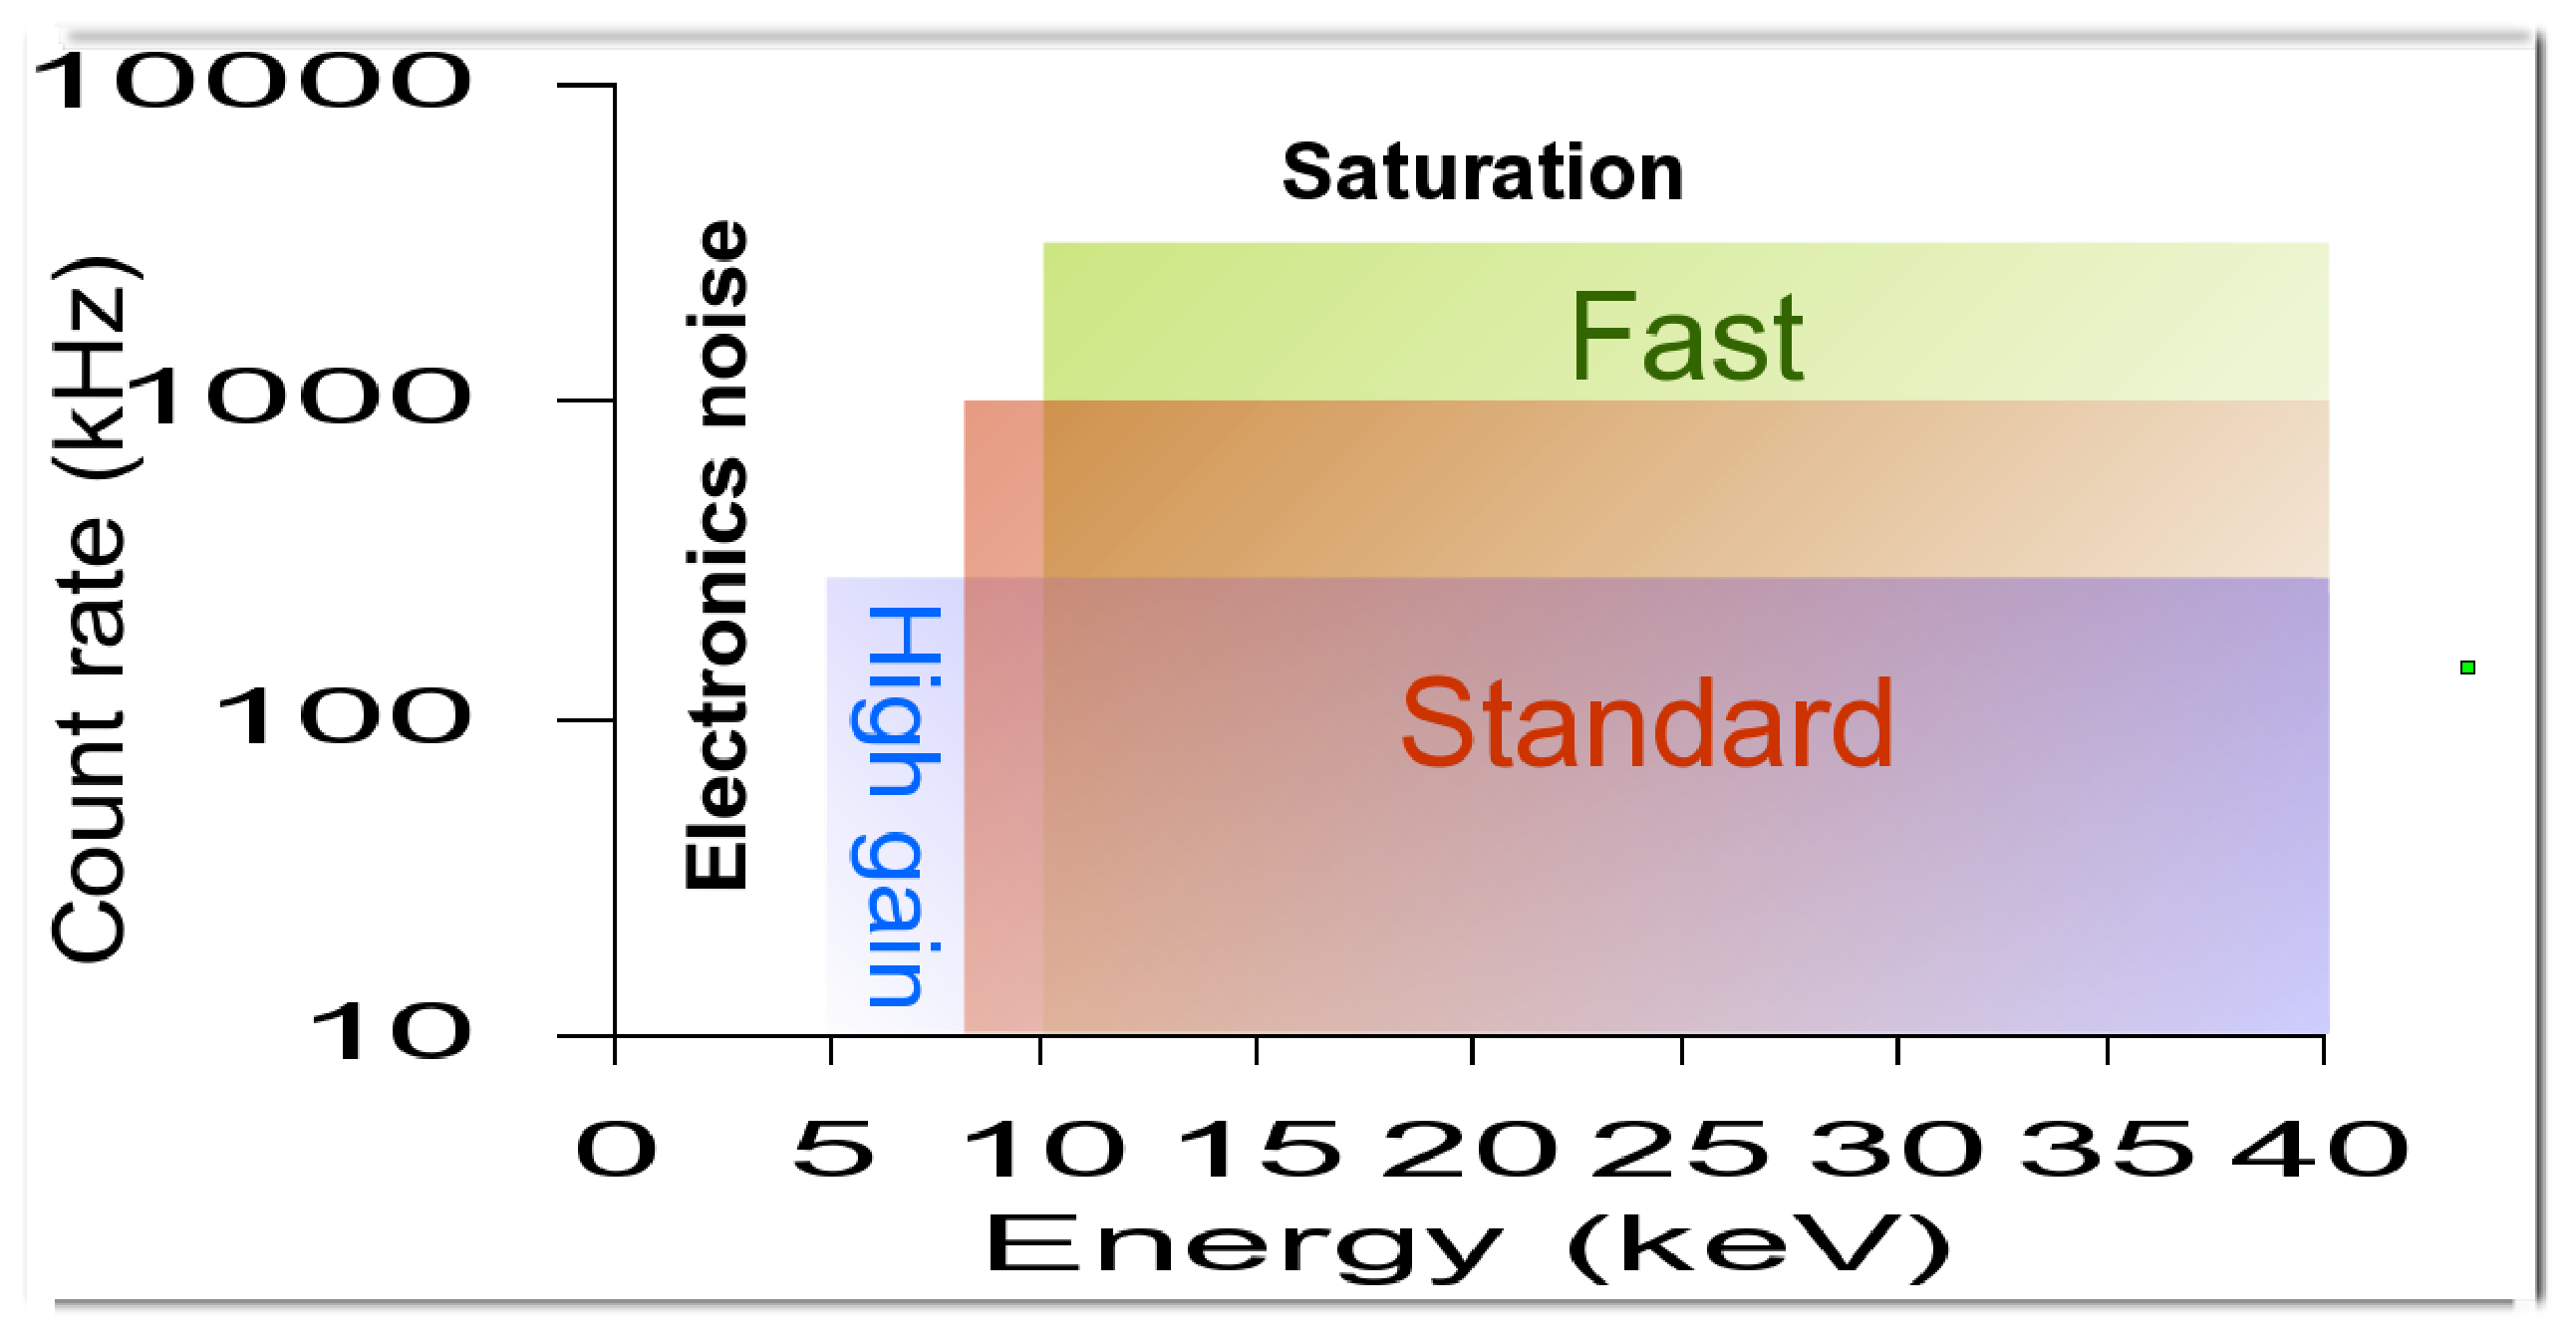
\includegraphics[width=\textwidth]{images/settings}
\end{figure} 

%\section{What is the electronic noise?}\label{sec:noise}


\section{What limits the maximum frame rate?}

In order to acquired the data, they should be:
\begin{itemize}
\item Transferred from readout electronics to readout board memory. This readou time is very dependent on the detector and on the dynamic range chose (for single photon counting detectors if configurable) and can range from hundreds or tens to few us. \\
In case the board has some memory that can be accessed by the hardware, this is the only limitation on the maximum frame rate as long as the memory is not filled (burst mode). Frame rates as high as a few tens of kHz can be achieved for photon countign detectors (EIGER) or up to 1~MHz for charge integrating (GOTTHARD).

\item Transferred from readout board to client PC or file server. In this case the main bottleneck is normally given by the data transfer rate on the network and on the performances of the receiver PC. This limits the frame rate in continous mode. However also the data writing capabilities and amount of data which are being acquired should be taken into consideration when setting up very fast acquisitions.

\end{itemize}

